\chapter{DESENVOLVIMENTO}

\section{Componentes de um diodo}

O diodo é um componente que possui 2 terminais, sendo eles: (i) catodo, e (ii) anodo. O catodo é o terminal negativo do diodo, e o anodo é o terminal positivo do diodo. A figura \ref{fig:componentes_diodo} mostra a representação esquemática de um diodo.

\begin{figure}[H]
    \centering
    \fbox{
        \parbox{0.975\textwidth}{
            \centering
            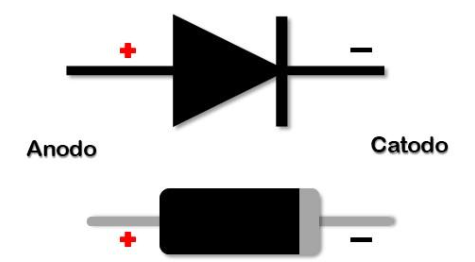
\includegraphics[width=0.975\textwidth]{images/componentes_diodo.png}
        }}
    \caption{Componentes do diodo}
    \vspace{-0.3cm}
    \label{fig:componentes_diodo}
\end{figure}

O simbolo na qual representa um diodo, é um triangulo, na qual o lado maior do triangulo representa o anodo, e o lado menor representa o catodo, que podem ser analisados através da imagem acima.

\section{Diodo ideal}

O funcionamento de um diodo ideal é simples: Ou ele está com uma chave fechada, ou ele está com uma chave aberta. Quando o diodo está com a chave fechada, ele permite a passagem de corrente elétrica, com Rd = 0, e quando o diodo está com a chave aberta, ele não permite a passagem de corrente elétrica, com Rd = $\infty$. A figura \ref{fig:diodo_ideal} mostra a representação esquemática de um diodo ideal.

\begin{figure}[H]
    \centering
    \fbox{
        \parbox{0.975\textwidth}{
            \centering
            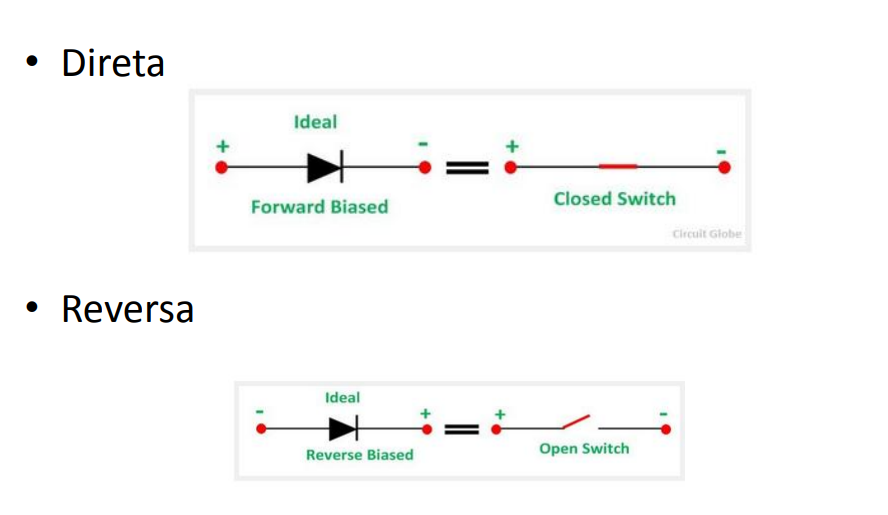
\includegraphics[width=0.975\textwidth]{images/diodo_ideal_polarizacao.png}
        }}
    \caption{Polarização de um diodo ideal}
    \vspace{-0.3cm}
    \label{fig:diodo_ideal}
\end{figure}

\subsection{Primeiro Circuito}

Com este conhecimento sobre diodo ideal, podemos encontrar a corrente e a tensão do circuito, que é mostrado na figura \ref{fig:ex_diodo_ideal_01}.

\begin{figure}[H]
    \centering
    \fbox{
        \parbox{0.975\textwidth}{
            \centering
            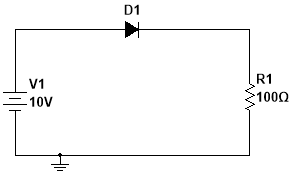
\includegraphics[width=0.975\textwidth]{images/circuito_01.png}
        }}
    \caption{Circuito 01}
    \vspace{-0.3cm}
    \label{fig:ex_diodo_ideal_01}
\end{figure}

\noindent
\textbf{Resolução}

\begin{Resolucao}[H]
    \fbox{
        \parbox{0.975\textwidth}{
            \vspace{0.40cm}
            \centering
            Com o diodo polarizado\dots
            \[I = \frac{V}{R} \rightarrow \frac{10}{100} = \textcolor{red}{0.1A} \]
            \[V =\textcolor{red}{ 10V} \]

            Com polarização reversa no diodo\dots
            \[ID = 0 \rightarrow \textnormal{(Pois o diodo não deixa passar corrente)}\]
            \[Vd = -10V\]
            \[Vo = 0\]
            \[Io = 0\]
        }
    }
    \captionof*{Resolucao}{Resolução: Circuito 01}
    \label{res:Circuito01}
\end{Resolucao}

Através da imagem \ref{fig:SimulacaoCircuito01} podemos verificar os resultados obtidos por simulação de díodo conduzindo. Observe que para realizar a simulação corretamente do diodo polarizado, foi removido o doido ideal, pois o seu funcionamento em um circuito é composto por uma chave fechada.

\begin{figure}[H]
    \centering
    \fbox{
        \parbox{0.975\textwidth}{
            \centering
            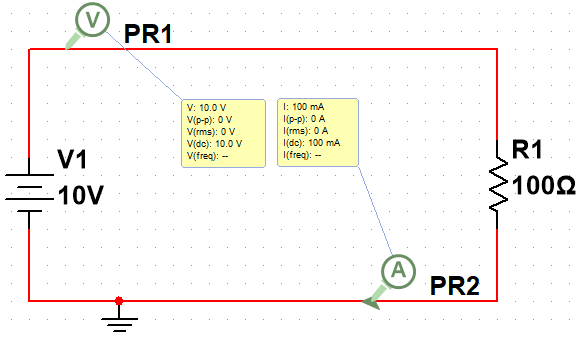
\includegraphics[width=0.975\textwidth]{images/simulacoes/circuito_01.png}
        }}
    \caption{Simulação do circuito 01}
    \vspace{-0.3cm}
    \label{fig:SimulacaoCircuito01}
\end{figure}

Com a tabela \ref{tab:Comparacao1Circuito} podemos comparar os resultados obtidos por simulação com os resultados obtidos por cálculo, na qual comprovam que os cálculos estavam corretos.

\begin{quadro}[H]
    \centering
    \caption{Comparação entre os resultados obtidos por simulação e os resultados obtidos por cálculo do circuito 01}
    \begin{tabular}{|C{0.34\textwidth}|C{0.19\textwidth}|C{0.19\textwidth}|C{0.19\textwidth}|C{0.19\textwidth}|}
        \hline
        \rowcolor[HTML]{C0C0C0}
        \textbf{Modelo\textbackslash{}Variáveis} & \textbf{I} & \textbf{V}\\
        \hline
        Calculado & 10mA & 10V \\
        \hline
        Simulado & 10mA & 10V \\
        \hline
    \end{tabular}
    \vspace{-0.6cm}
    \label{tab:Comparacao1Circuito}
\end{quadro}

\subsection{Segundo Circuito}

Após ser estudado este primeiro circuito, podemos estudar o segundo circuito, que é mostrado na figura \ref{fig:ex_diodo_ideal_02}.

\begin{figure}[H]
    \centering
    \fbox{
        \parbox{0.975\textwidth}{
            \centering
            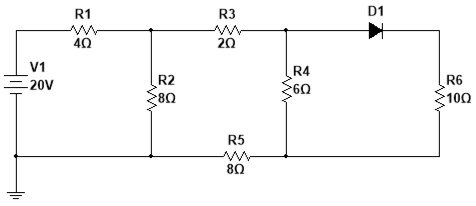
\includegraphics[width=0.975\textwidth]{images/circuito_02.png}
        }}
    \caption{Circuito 02}
    \vspace{-0.3cm}
    \label{fig:ex_diodo_ideal_02}
\end{figure}

\begin{Resolucao}[H]
    \fbox{
        \parbox{0.975\textwidth}{
            \vspace{0.40cm}
            \centering
            Para realizar a análise deste circuito, o mesmo será simplificado através de Thevenin
            \[\textnormal{Resistor Equivalente: }  ((4 // 8) + (2 + 8)) // 6 = \textcolor{red}{4.07\Omega} \]
            Para encontrar Vth\dots
            \[x = \frac{16*8}{16+8} \simeq 5.33\]
            \[\textnormal{Utilizando divisor de tensão\dots} x = \frac{5.33}{4 + 5.33} \]
            \[x * 20 \simeq \textcolor{red}{11.42V}\]
            \[\frac{6}{8 + 6 + 2} * 11.42 \simeq \textcolor{red}{4.28V} \]
            \[IT = \frac{4.28}{4.07 + 10} \simeq \textcolor{red}{0.304A}\]
            \[VRL = 0.304 * 10 \simeq \textcolor{red}{3.04V}\]
        }
    }
    \captionof*{Resolucao}{Resolução: Circuito 02}
    \label{res:Circuito01}
\end{Resolucao}

Após os cálculos acima, obtemos o circuito de Thévenin, demonstrado na imagem \ref{fig:thevenin_circuito_01}.

\begin{figure}[H]
    \centering
    \fbox{
        \parbox{0.975\textwidth}{
            \centering
            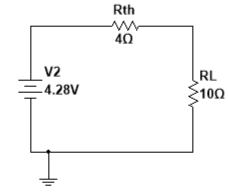
\includegraphics[]{images/thevenin_circuito_01.png}
        }}
    \caption{Circuito 02}
    \vspace{-0.3cm}
    \label{fig:thevenin_circuito_01}
\end{figure}

Através da imagem \ref{fig:SimulacaoCircuito04} podemos verificar os resultados obtidos por simulação. 

\begin{figure}[H]
    \centering
    \fbox{
        \parbox{0.975\textwidth}{
            \centering
            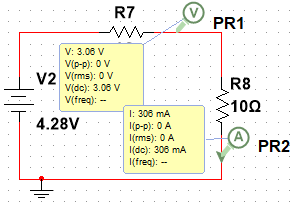
\includegraphics[width=0.975\textwidth]{images/simulacoes/circuito_04.png}
        }}
    \caption{Simulação do circuito 03}
    \vspace{-0.3cm}
    \label{fig:SimulacaoCircuito04}
\end{figure}

Com a tabela \ref{tab:Comparacao1Circuito04} podemos comparar os resultados obtidos por simulação com os resultados obtidos por cálculo, na qual comprovam que os cálculos estavam corretos, mas tiveram uma pequena variação, devido a aproximação de valores nos cálculos.

\begin{quadro}[H]
    \centering
    \caption{Comparação entre os resultados obtidos por simulação e os resultados obtidos por cálculo do circuito 01}
    \begin{tabular}{|C{0.34\textwidth}|C{0.19\textwidth}|C{0.19\textwidth}|C{0.19\textwidth}|C{0.19\textwidth}|}
        \hline
        \rowcolor[HTML]{C0C0C0}
        \textbf{Modelo\textbackslash{}Variáveis} & \textbf{VRL} & \textbf{IRL}\\
        \hline
        Calculado & 3.04V & 0.304A \\
        \hline
        Simulado & 3.06V & 0.306A \\
        \hline
    \end{tabular}
    \vspace{-0.6cm}
    \label{tab:Comparacao1Circuito04}
\end{quadro}

\subsection{Circuito 02 com fonte invertida}

Invertendo a fonte do circuito \ref{fig:ex_diodo_ideal_02}, sabemos que o diodo irá ser polarizado reversamente, ou seja, terá seu funcionamento como uma chave aberta. A imagem \ref{fig:ex_diodo_ideal_02_reverso} mostra o circuito com a fonte invertida.

\begin{figure}[H]
    \centering
    \fbox{
        \parbox{0.975\textwidth}{
            \centering
            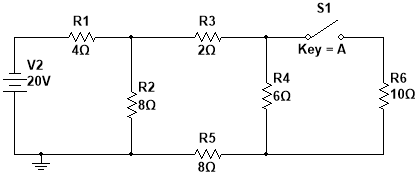
\includegraphics[width=0.975\textwidth]{images/circuito_03.png}
        }}
    \caption{Circuito 02 com fonte invertida}
    \vspace{-0.3cm}
    \label{fig:ex_diodo_ideal_02_reverso}
\end{figure}

Podemos afirmar então, que por motivos de ter uma chave aberta neste local, IR1 e VR1 são 0V, já Vd possui valor de -20V.

\section{Comportamento de um diodo}

\begin{figure}[H]
    \centering
    \fbox{
        \parbox{0.975\textwidth}{
            \centering
            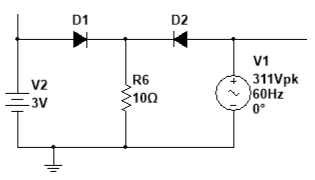
\includegraphics[width=0.975\textwidth]{images/circuito_04.png}
        }}
    \caption{Circuito 03}
    \vspace{-0.3cm}
    \label{fig:circuito_04}
\end{figure}

No circuito da imagem \ref{fig:circuito_04}, podemos observar que existem 2 diodos e duas fontes, na qual V1 é AC e V2 é DC. Sabemos qeu quando V1 estiver no semi ciclo negativo, o diodo não irá conduzir, tendo em sua carga, somente a contribuição dada por V2. Quando V1 estiver no semi ciclo positivo, o diodo irá conduzir, tendo em sua carga, a contribuição dada por V1 e V2, gerando uma forma de onda como a mostrada a partir da imagem \ref{fig:forma_de_onda_circuito_04}

\begin{figure}[H]
    \centering
    \fbox{
        \parbox{0.975\textwidth}{
            \centering
            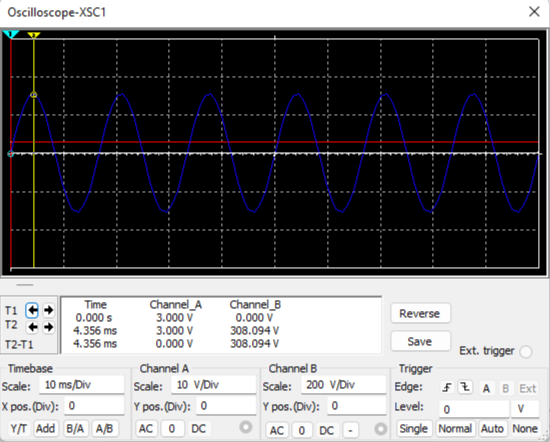
\includegraphics[width=0.975\textwidth]{images/forma_de_onda_circuito_04.png}
        }}
    \caption{Circuito 02 com fonte invertida}
    \vspace{-0.3cm}
    \label{fig:forma_de_onda_circuito_04}
\end{figure}

Através da forma de onda, é possível perceber a forma de onda das duas fontes. Sendo a linha vermelha representada pela fonte V2, e a linha azul representada por V1. Note que quando a fonte V1 atingir a tensão menor que 3V, a tensão na carga passa a ter somente a contribuição da fonte V2. Ou seja, a tensão na carga terá somente o semi ciclo positivo da fonte V1, quando a fonte de tensão for superior a 3V.